%\documentclass[a4paper,11pt,twoside]{article}
%\usepackage{graphicx}
%\begin{document}

\begin{figure}[h]
	\centering
	
\includegraphics[width=0.5\linewidth]{Grafik/Diagramm/Pattern/ClientServer/Kontext.png}
	\caption[]{Client-Server-Modell}
\end{figure}

\paragraph{Client}
Der Client ist der für den Nutzer sichtbare Teil des Systems, also die Website, über die auf die serverseitigen Anwendungen zugegriffen werden kann.

\paragraph{Server}
Der Server bietet dem Nutzer den Dienst an Modelle anhand von schon vorhandenen oder von ihm hochgeladenen Datensätzen und Algorithmen zu erstellen. Hierzu verwaltet der Server eine Datenbank, die entsprechende Nutzerdaten, Modelle und Algorithmen beinhaltet.\\

\begin{figure}[h]
	\centering
	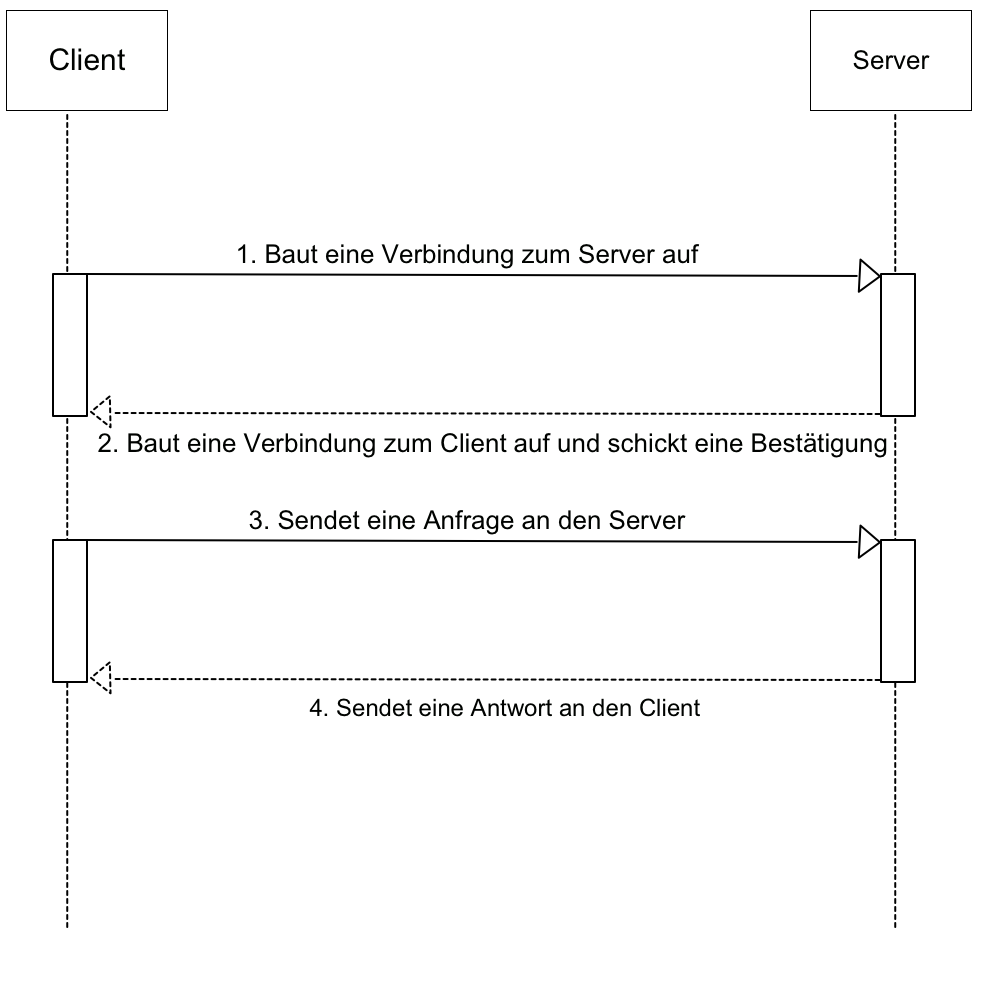
\includegraphics[width=0.6\linewidth]{Grafik/Diagramm/Pattern/ClientServer/Sequenzdiagramm.png}
	\caption[]{Client-Server-Sequenzdiagramm}
\end{figure}\pagebreak
\noindent Der Client versucht eine Verbindung zum Server aufzubauen. Der Server versucht ebenfalls bei Anfrage eine Verbindung zum Client aufzubauen und schickt diesem eine Bestätigung, dass die Kommunikation erfolgen kann. Danach kann der Client Datensätze und Algorithmen hochladen und dem Server eine Anfrage zum Modelle berechnen oder downloaden schicken.
\subsubsection{Was spricht für das Client-Server-Modell?}
Das Client-Server-Modell wird verwendet, wenn eine Datenbank oder ein Service von verschiedenen Orten her abrufbar sein soll. Für unser System sind beide dieser Aspekte gegeben. Verschiedene Nutzer können so als Client auf das System zugreifen und Daten hoch- und runterladen. Änderungen am System können rein serverseitig erfolgen ohne Zutun oder Benachrichtigung des Clients, was zu einer erhöhten Flexibilität und Stabilität führt.\\
Da das System über das REST-Protokoll mehrere Server adressieren können soll, ist es mehr als sinnvoll das Client-Server-Pattern zu verwenden, da andernfalls eine Implementierung dieses Protokolls nur schwer realisierbar wäre. 




%\end{document}